\documentclass[a4paper,twocolumn]{report}

% -- TOC --
\usepackage[nottoc,section,numbib]{tocbibind}
\usepackage[titles]{tocloft}

% -- Typography --
\usepackage[utf8]{inputenc}
\usepackage{microtype}

% -- Fonts --
%\usepackage{charter}
%\usepackage{palatino}

% -- Math --
\usepackage{amsmath}

% -- Tables --
\usepackage{booktabs}

% -- Graphics --
\usepackage{pgfplots}

% -- Misc. --
\usepackage{hyperref}
\usepackage{color}
\usepackage{array}
\usepackage{url}

\title{Internal Assessment\\
    Replication of Loftus and Palmer (1974)}
\author{Siddharth Mahendraker\\
    Psychology HL\\
    Word Count: 1418\\}

\begin{document}
\maketitle

\begin{abstract}
This paper investigates the influence of leading questions on memory by
replicating the famous study conducted by Loftus and Palmer in 1974. After
watching a video of a car crash, participants are asked a leading question
wherein the verb describing the collision is controlled (“smashed”, “hit”).
The question asks the participants to estimate the speed of the collision
(and hence recall it from memory). The results indicate that the schemata
associates with the verb in the leading question influence the recall of
the event, and result in an inaccurate reconstruction of the memory. More
specifically, mild verbs such as “hit” resulted in lower speed estimates,
while more intense verbs such as “smashed” elicited higher speed estimates.
As in the original study, these results support the conclusion that leading
question do indeed have a significant influence on memory, specifically
recall, as they introduce new information which may trigger certain schemata
and hence interfere with memory retrieval.
\end{abstract}

% -- Bookkeeping
\setcounter{secnumdepth}{3}
\renewcommand{\thesection}{\arabic{section}}
\renewcommand{\cftsecfont}{\bfseries}
\settocbibname{References}
\setlength\cftbeforesecskip{3pt}
\setlength\cftbeforesubsecskip{3pt}

% -- Easier footnotes
\newcounter{fn}
\newcommand{\fnt}[1]{%
\addtocounter{fn}{1}%
\footnote[\value{fn}]{#1}}

% -- ToC --
\setcounter{page}{1}
\pagenumbering{roman}
\tableofcontents
\clearpage
\setcounter{page}{1}
\pagenumbering{arabic}

\section{Introduction}

Memory is the cognitive process which deals with the storage and retrieval
of information. It is well known that memory, particularly the retrieval of
memory, is terribly inaccurate. That is, memory does a very poor job of
storing and retrieving the exact information we’re trying to remember. The
inaccurate nature of memory was first rigorously accounted for by Bartlett
in 1932 \cite{bartlett}. He suggested that rather than record information,
memory is actually a reconstructive process; new information is processed
according to information we already know. This pre-known information is
stored in mental structures called schemata, which provide a framework for
organizing information.

Based on his ideas, Bartlett claimed that memory distortions were due to
information being processed through our personal and cultural schemata. He
investigated this claim by conducting an experiment. English participants
were asked to serially reproduce an Aboriginal story which contained many
elements specific to Aboriginal culture. Unfamiliar with the style of the
story, participants’ memory of the story quickly changed to accommodate
their cultural schemes; the story became shorter, details deemed
insignificant by the englishmen were removed and new more conventional
details were added. In turn, these results supported Bartlett’s idea of
reconstructive memory based on schemes.

Based on the idea of reconstructive memory influenced by previously known
information, Loftus and Palmer wanted to find out whether the use of leading
questions (questions which suggest an answer) could affect recall. In a
study conducted in 1974 \cite{lap}, the researchers performed an experiment wherein
participants were shown footage of two cars colliding and were asked a
leading question about the speed of the collision. The leading question contained a
controlled verb describing the incident (“contacted”, “hit”, “smashed”). It
was found that the verb used had a significant effect on the speed estimate.
More specifically, dramatic verbs such as “smashed” elicited high speed
estimates, while milder verbs such as “contacted” elicited low speed
estimates. This seems to indicate that leading questions do indeed influence
the retrieval of memory; the schemata evoked by the control verb interfere
with the retrieval of information about the event.

In this paper, we attempt to replicate Loftus and Palmer with the same aim;
to investigate whether leading questions affect memory retrieval.

\section{Method}

\subsection{Apparatus}

\begin{itemize}
\item Consent form
\item Debriefing form
\item Video of car crash
\item Questionnaire with the “hit” condition
\item Questionnaire with the “smashed” condition
\item Computer
\end{itemize}

See the Appendix, subsection 1 for more information.

\subsection{Procedure}

To make sure ethical procedures were being followed, participants signed a
consent form and were verbally reminded about their rights before the
experiment had begun.

Participants were then individually guided into a quiet room and seated in
front of a computer. A segment of a video depicting car crashes was shown
to each participant. The video itself was part of a compilation of car
crash videos obtained from around Europe. Each participant only saw the
video segment once. The clip was 8 seconds long, and featured an accident
between a car turning onto the road and another car coming in from the right.
After watching the clip, participants were asked to fill out a randomly
chosen questionnaire, which asked them a variety of specific questions about
the accident.

After the experiment was over, participants were verbally de-briefed and
given a debrief form which explained the objectives of the experiment in
greater detail.

\subsection{Design}

To allow for a controlled environment and to establish a clear cause and
effect relationship, a laboratory experiment design was used. The
independent variable is the verb used in the critical question of the
questionnaire. The dependant variable is the estimate of the speed of the
cars in the witnessed collision, as an answer to the critical question in
the questionnaire.

In an attempt to avoid demand characteristics, 4 extra questions were added
to the questionnaire to shift the focus away from the critical question
regarding the speed estimate. Furthermore, to reduce experimenter’s bias
(esp. resulting from the use of opportunity sampling), the study was
conducted using a double blind design. Questionnaires containing the two
verbs used as the independent variables (“hit”, “smashed”) were shuffled in
a random order, and then distributed to participants in a random fashion.
Neither the experimenter nor the participant knows the value of the
independent variable until after the experiment is over.

Ethical guidelines were also stringently followed. Before the experiment,
participants signed consent forms wherein they were made aware that their
data will be kept confidential, that no personal data or information will
be taken and that they have the right to withdraw themselves and their data
from the study at any time. Participants were also debriefed after the
experiment and reminded of their aforementioned rights.

\subsection{Participants}

In order to quickly and easily gather data, an opportunity sample was used.
Participants were chosen from the population of grade 11 and 12 student at
school who don’t take psychology. This prevented students who were familiar
with the study from participating. Ten participants were chosen in total,
all of whom agreed to participate in the study. The participants were
randomly split into two experimental groups based on the questionnaires
they received.

\section{Results}

The responses to the questionnaire were tabulated and the central tendency
and dispersion of the results were calculated. Of the 10 questionnaires
returned, 6 responded to the “smashed” condition and 4 responded to the
“hit” condition. The mean speed estimated in the “hit” condition was 40
km/hr, with estimates ranging from 30-50 km/hr (a range of 20 km/hr).
In contrast, the mean speed estimated in the “smashed” condition was
significantly higher at 60 km/hr, with a much wider dispersion ranging from
40-90 km/hr (a range of 50 km/hr).

The mean estimated speeds describe the average speed estimates of the
participants and the ranges describe how spread apart (or how close)
the various data points were.

This same information has been graphed and tabulated below.

\begin{figure}[h]
\begin{center}
\begin{tabular}{ccc}
\toprule
Condition & Mean (km/hr) & Range (km/hr)\\
\midrule
“hit” & 40 & 20\\
“smashed” & 60 & 50\\
\bottomrule
\end{tabular}
\end{center}
\caption{Mean and range results for “hit” and “smashed” conditions.}
\end{figure}

\begin{figure}[h]
\begin{center}
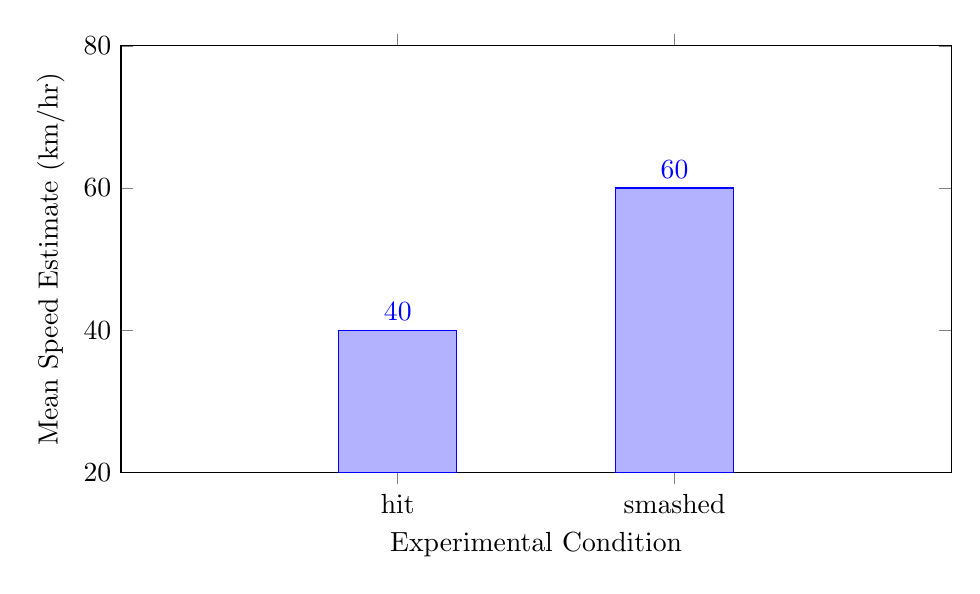
\begin{tikzpicture}
    \begin{axis}[
        ybar,
        width={\columnwidth},
        height=7cm,
        ylabel={Mean Speed Estimate (km/hr)},
        xlabel={Experimental Condition},
        symbolic x coords={hit,smashed},
        enlargelimits=1.0,
        bar width=1.5cm,
        xtick=data,
        nodes near coords,
        nodes near coords align={vertical},
        x tick label style={anchor=north}]
    \addplot coordinates {(hit, 40) (smashed,60)};
    \end{axis}
\end{tikzpicture}
\end{center}
\caption{Comparison of mean speed estimates.}
\end{figure}

The results clearly show a difference between the speed estimates in the
two experimental conditions. The mean speed estimates in the “smashed”
condition are 50\% higher than the mean speed estimates in the “hit”
condition.

See the Appendix, subsection 2 for the raw data and calculations.

\section{Discussion}

The result of our experiment clearly suggest that the use of leading
questions does indeed influence memory. As in the original study conducted
by Loftus and Palmer, the mean speed estimate was significantly higher in
the “smashed” condition than in the “hit” condition. Based on the
reconstructive theory of memory proposed by Bartlett, these results could
be explained due to the triggering of the schemata associated with the
respective verbs “smashed” and “hit”. The intense, dramatic schema
associated with the word “smashed” elicited higher speed estimates, while
the milder, less intense schema associate with the word “hit” elicited
lower speed estimates.

In conclusion, extra information obtained from the schemata associated with
the verb in the leading question interfered with the retrieval of memory,
causing differing mean speed estimates in the two experimental conditions.
This conclusion closely resembles that of Loftus and Palmer, who also
showed that the schema associated with the verb used in the leading question
interfered with memory retrieval.

Despite the solid conclusions we were able to draw, this experiment suffers
from several limitation both in it’s design and it’s procedure. Firstly,
the extremely small sample size and the use of opportunity sampling
introduced significant bias to the results, as not every stratum of the
population was represented. Furthermore, although a double blind design was
used, the experimenter (due to the sampling method used) may have
inadvertently chosen participants who were more likely to give answers he
expected or wanted. As in the original study, the experiment lacked
ecological validity, as participants were shown a video of a car crash
rather than the real thing. In the real life event, they might have been
able to assimilate more information about the crash, perhaps even enough
information to disregard the extra information communicated in the leading
question. Furthermore, the quality of the video of the car crash was far
less than ideal; unlike our eyes and ears, the image wasn’t very high
resolution and the sound was fair. Therefore, the net information
communicated in the video was far less than what would have been
communicated in real life. Lastly, the experiment does not directly
address the fact that these verbs have interfered with the recall of the
memory of the car crash, rather, it only shows that these verbs interfered
with the recall of the speed at which the crash occurred. To ascertain
whether the real memory of the crash were affected, I would have to test
whether other elements likely to be associated with the verb’s schema were
present in the participants’ memories. Otherwise, it could be argued that
the extra information communicated in the leading question helped the
participant choose a more accurate speed, and no memory was really altered.
In the original study conducted by Loftus and Palmer, a second experiment
was used to establish the fact that the memory was truly modified.

Conducting this experiment over, I would definitely expand the sample
population and use a less biased sampling method, such as random sampling.
This would reduce the bias introduced by the small population and allow the
findings of the study to easily generalize. The ecological validity of the
experiment could also be improved by attempting to use real life car
accidents and accident witnesses, however, this remains difficult and
dangerous.

\bibliographystyle{plain}
\bibliography{doc.bib}

\clearpage
\section{Appendix}

\subsection{Materials and Apparatus}

\begin{figure}[h]
\begin{center}
\begin{tabular}{cc}
\toprule
Item & URL\\
\midrule
Consent form & \url{http://bit.ly/VKofDc}\\
Debriefing form & \url{http://bit.ly/YHO7gc}\\
Video of car crash & \url{http://bit.ly/11Rrb2O}\\
Questionnaires & \url{http://bit.ly/Xrwn5T}\\
\bottomrule
\end{tabular}
\end{center}
\caption{URL locations of the materials used in this study.}
\end{figure}

\subsection{Raw Data and Calculations}

\begin{figure}[h]
\begin{center}
\begin{tabular}{ccc}
\toprule
Participant & Speed Estimate & Condition\\
\midrule
1 & 50 & hit\\
2 & 40 & hit\\
3 & 30 & hit\\
4 & 40 & hit\\
5 & 70 & smashed\\
6 & 90 & smashed\\
7 & 40 & smashed\\
8 & 50 & smashed\\
9 & 60 & smashed\\
10& 50 & smashed\\
\bottomrule
\end{tabular}
\end{center}
\caption{Raw data of both experimental conditions.}
\end{figure}

The mean for both experimental conditions was calculated using the following
formula,
\begin{align*}
    \mu = \frac{1}{n}\sum{x}.\\
\end{align*}
Therefore,
\begin{align*}
    \mu_{\text{hit}} &= \frac{1}{4}\sum{x}\\
    &= \frac{1}{4} \cdot 160\\
    &= 40.
\end{align*}
And,
\begin{align*}
    \mu_{\text{smashed}} &= \frac{1}{6}\sum{x}\\
    &= \frac{1}{6} \cdot 360\\
    &= 60.
\end{align*}

The range for both experimental conditions was calculated using the following
formula,
\begin{align*}
    \text{range} = \max{x} - \min{x}.
\end{align*}
Therefore,
\begin{align*}
    \text{range}_{\text{hit}} &= \max{x} - \min{x}\\
    &= 50 - 30\\
    &= 20.
\end{align*}
And,
\begin{align*}
    \text{range}_{\text{smashed}} &= \max{x} - \min{x}\\
    &= 90 - 40\\
    &= 50.
\end{align*}

\end{document}
